% =====================================================================
\section{Data and forecast-sample construction}\label{sec:data}

\subsection{The GDP hourly product}
We use version 2.01 of the GDP hourly dataset \citep{gdpdata2022}. Each record gives a drifter identifier, UTC time, longitude $\lambda$, latitude $\phi$, eastward and northward velocity $(u,v)$ in \si{m\,s^{-1}}, SST, and a drogue-status flag. Two properties of the product matter for interpretation. First, positions and velocities on the hourly grid are \emph{estimates} obtained by fitting irregular satellite fixes, not direct hourly measurements. The fit at time $t$ draws on fixes on either side of $t$ \citep{elipot2016}, so the velocity at a forecast origin carries a small amount of information from the following hours. Second, most drifters eventually lose their drogue, after which wind slip makes the recorded velocity no longer representative of the \SI{15}{m} current. The final cohort was not filtered on drogue status.

\subsection{Cohort definition}
Forecast origins were restricted to the box \ang{80}--\ang{60}W, \ang{30}--\ang{45}N and to July--September of 2007--2022 (\cref{fig:region}a). Historical inputs and targets were allowed to fall outside the box or season; for example, a 1~July origin may use 30~June history. All observations were retrieved from the complete trajectories of drifters that entered the region (\num{20216717} hourly records).

A forecast case at origin $t$ requires (i) all 25 hourly records from $t-24$\,h to $t$ with valid position and velocity, and (ii) an observed position at exactly $t+24$\,h. Records were matched by drifter identifier and timestamp rather than by row offset, so gaps in a track cannot silently shift the horizon. Of \num{632770} eligible origins from 519 drifters, \num{626679} (99.04\%) from 517 drifters satisfied both requirements (\cref{tab:cohort}). Every method is evaluated on exactly the same cases, including the baselines that do not use history.

\begin{figure}[!htbp]
  \centering
  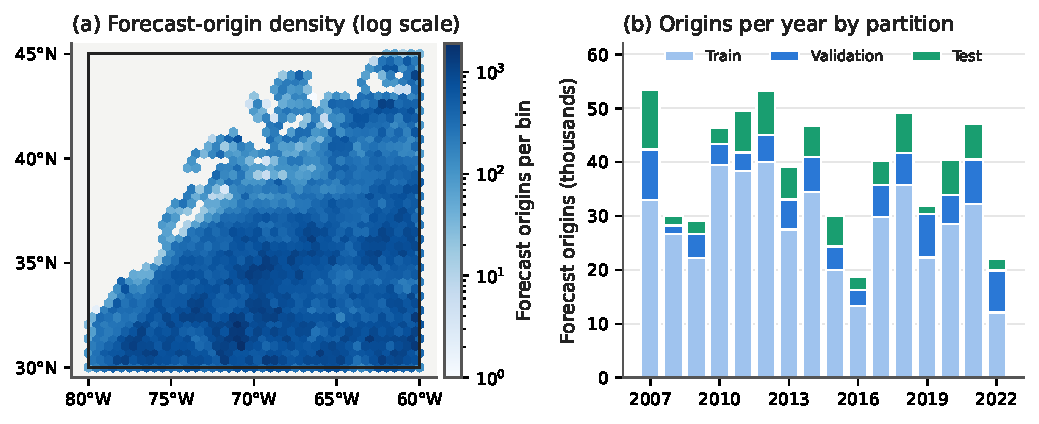
\includegraphics[width=\textwidth]{figures/generated/fig_study_region_coverage.pdf}
  \caption{Study region and sample coverage. (a) Density of the \num{626679} forecast origins (logarithmic colour scale); the black rectangle is the origin-selection box. Land and unsampled areas are blank; no coastline is drawn. (b) Number of forecast origins per year by drifter-disjoint partition. Between 25 and 54 distinct drifters contribute in each year. Generated from \texttt{modelling\_dataset\_final.parquet} (\cref{app:repro}).}
  \label{fig:region}
\end{figure}

\begin{table}[!htbp]
  \centering
  \caption{Forecast cohort and drifter-disjoint partitions. The split assigns whole drifters, so sample shares differ from the nominal 70/15/15 drifter shares. ``Undrogued'' is the share of forecast origins whose drogue-status flag is false at $t$, computed for this report as a descriptive check (not used by any model).}
  \label{tab:cohort}
  \small
  \begin{tabular}{lrrrr}
    \toprule
    Partition & Forecast cases & Share of cases & Drifters & Undrogued origins \\
    \midrule
    Training   & \num{455662} & 72.7\% & 361 & 48.2\% \\
    Validation & \num{88471}  & 14.1\% & 78  & 53.6\% \\
    Test       & \num{82546}  & 13.2\% & 78  & 46.0\% \\
    \midrule
    Total      & \num{626679} & 100\%  & 517 & 48.7\% \\
    \bottomrule
  \end{tabular}
\end{table}

\subsection{Data characteristics relevant to the analysis}
Recent motion in the cohort is strongly right-skewed. The 24-hour mean speed has median \SI{0.31}{m\,s^{-1}} and mean \SI{0.41}{m\,s^{-1}}, with a maximum of \SI{2.60}{m\,s^{-1}}. The mean turning rate has median \SI{9.4}{\degree\per\hour}. Sampling is uneven in space and time. Origins concentrate in the southern and central parts of the box, whereas the northern Gulf Stream extension is sparsely and patchily sampled (\cref{fig:region}a). Annual sample sizes vary by a factor of almost three (\cref{fig:region}b). Origin-time SST was available for 98.4\%, 97.0\% and 94.3\% of training, validation and test cases. Finally, 48.7\% of origins come from drifters flagged as undrogued (\cref{tab:cohort}). This proportion was identified only during report preparation; \cref{sec:limitations} discusses its consequences.
